\chapter{Organisation du travail}

\section{Rapports hebdomadaires}

\paragraph{} \hspace{10mm}
A chaque fin de semaine, j'ai réalisé un compte rendu hebdomadaire qui a permis de synthétiser le travail accompli pendant la semaine et de planifier les tâches à venir pour la semaine suivante. Cela m'a aidé à suivre mon avancement et de m'assurer que je restais en ligne avec les objectifs fixés. De plus, ces rapports ont permis à mon tuteur et à mon suiveur de connaître l'avancée de mon travail et de me fournir des conseils et des orientations pour la suite de mon stage.
\paragraph{} \hspace{10mm}
Ces comptes rendus ont également donné lieu à des réunions à des moments où un simple échange par mail ne pouvait pas suffire. Ces réunions ont permis de discuter en détail du travail à venir sur le moyen terme et des directions à prendre, ainsi que de faire des mises aux points concernant des questions plus approfondies. 
En somme, la réalisation de ces comptes rendus hebdomadaires et la participation à des réunions ont été des éléments clés de mon stage, me permettant de m'assurer que j'atteignais les objectifs fixés.

\section{Planning prévisionnel}

\paragraph{} \hspace{10mm}
Afin de mieux pouvoir imaginer le déroulement du stage, voici le planning prévisionnel montrant comment le développement du projet avait été pensé. Après discussions avec M. Gechter, nous nous étions fixés jusqu'à fin novembre pour terminer le travail sur le projet déjà existant avant de commencer les ontologies. On peut remarquer que la répartition du travail sur la fin du stage est assez floue car ne connaissant pas les ontologies, je ne savais pas à quoi m'attendre avant d'aborder ce sujet.
\begin{figure} [H]
    \centering
    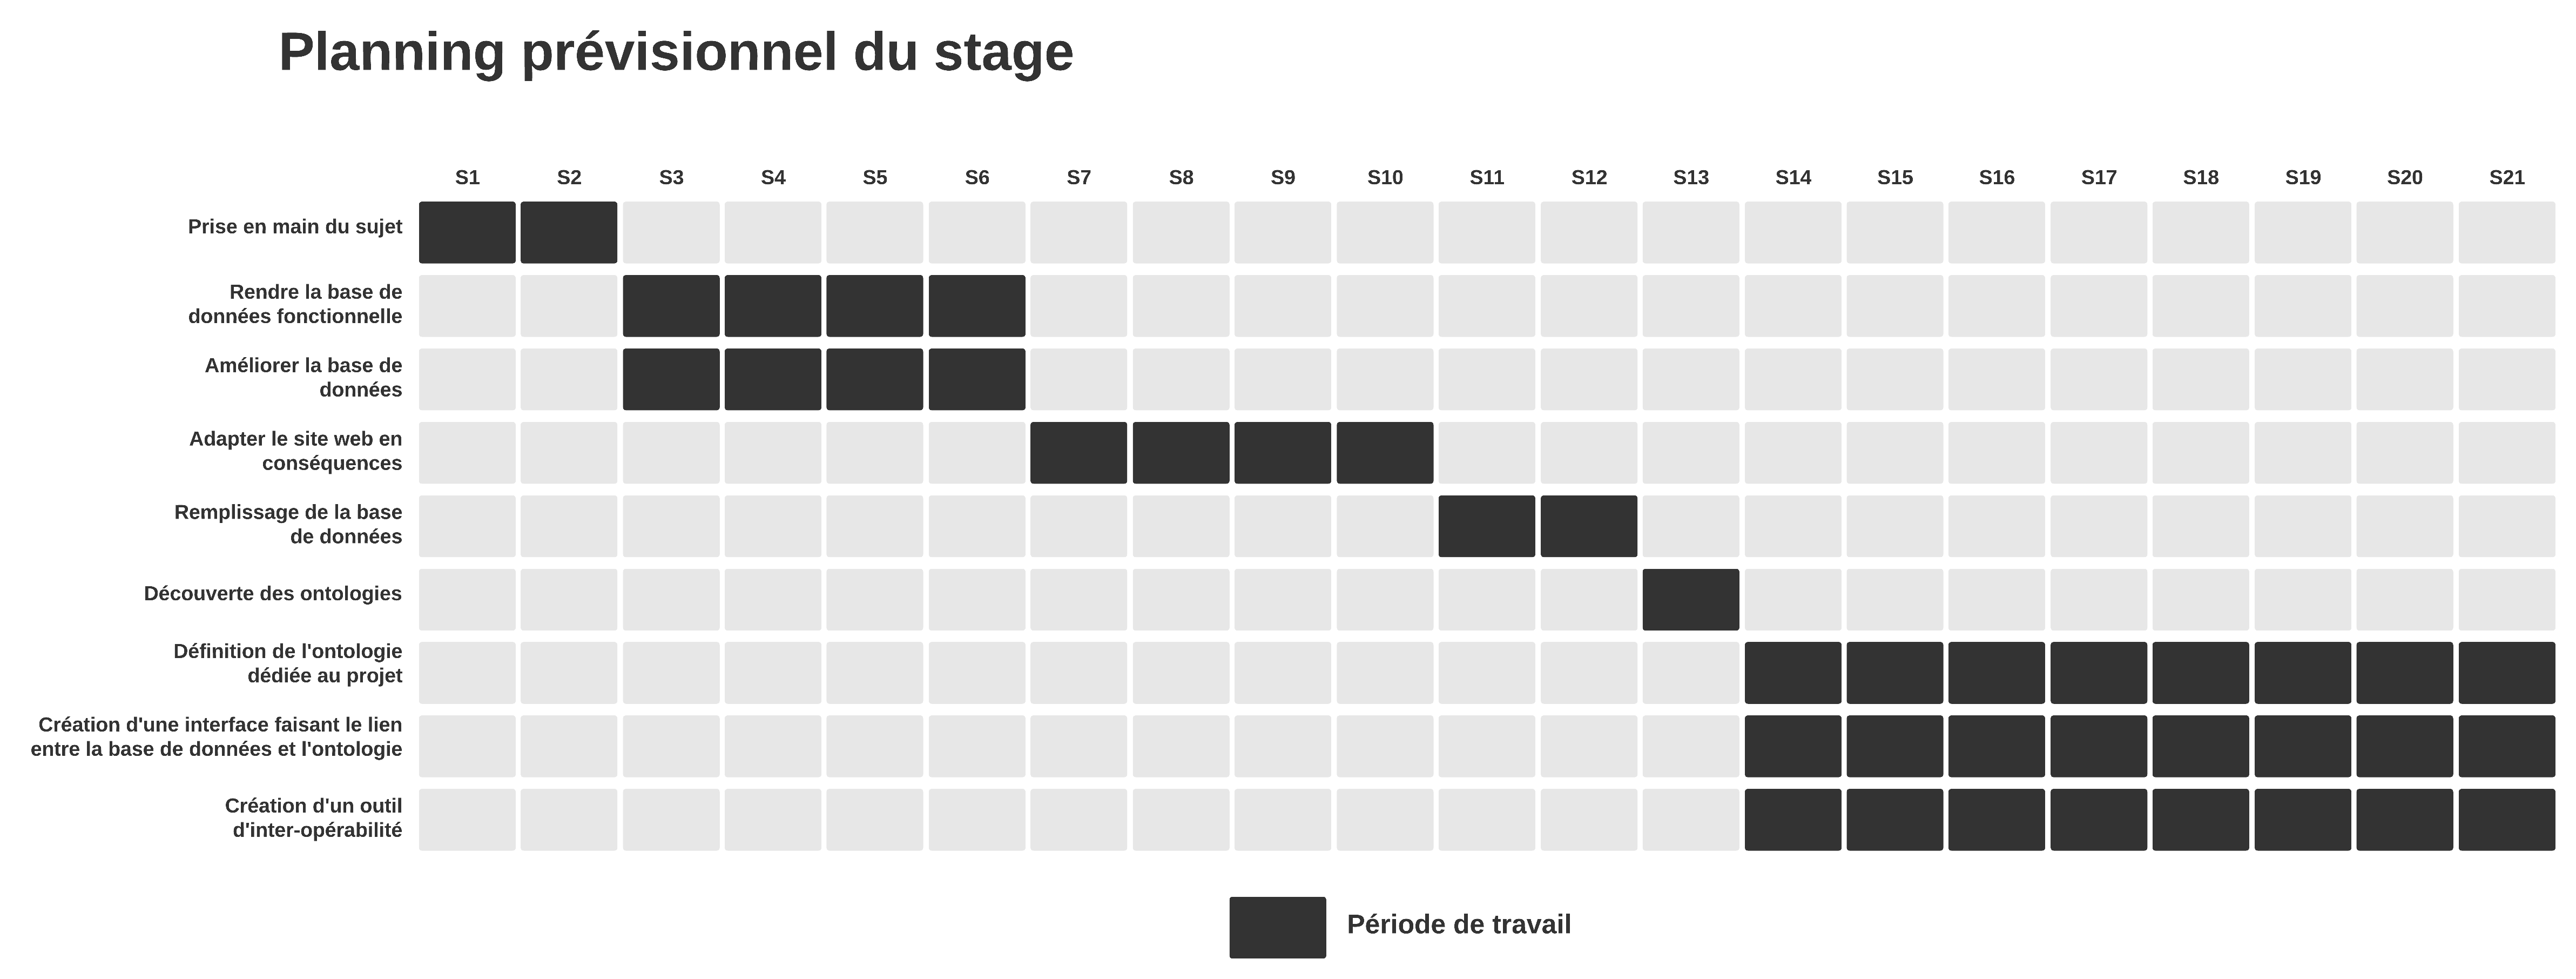
\includegraphics[width=1\textwidth]{assets/planning/planning_previsionnel.png}
    \caption{Planning prévisionnel}
    \label{fig:planningPrevisionnel}
\end{figure}

\section{Planning réel}

\paragraph{} \hspace{10mm}
En comparaison avec ce qui était prévu et ce que j'ai réellement pu faire, voici les plannings réels à la période de Noël et à la fin du stage. Après mon séjour à Nantes pour rencontrer Matthieu Quantin et Florent Laroche, nous avons réalisé que le projet existant posait de nombreux problèmes et qu'il était nécessaire de changer de voie. Nous avons dû corriger notre approche pour gérer le stockage des données liées au projet et cela a entraîné des modifications importantes dans le planning initial.

\begin{figure} [H]
    \centering
    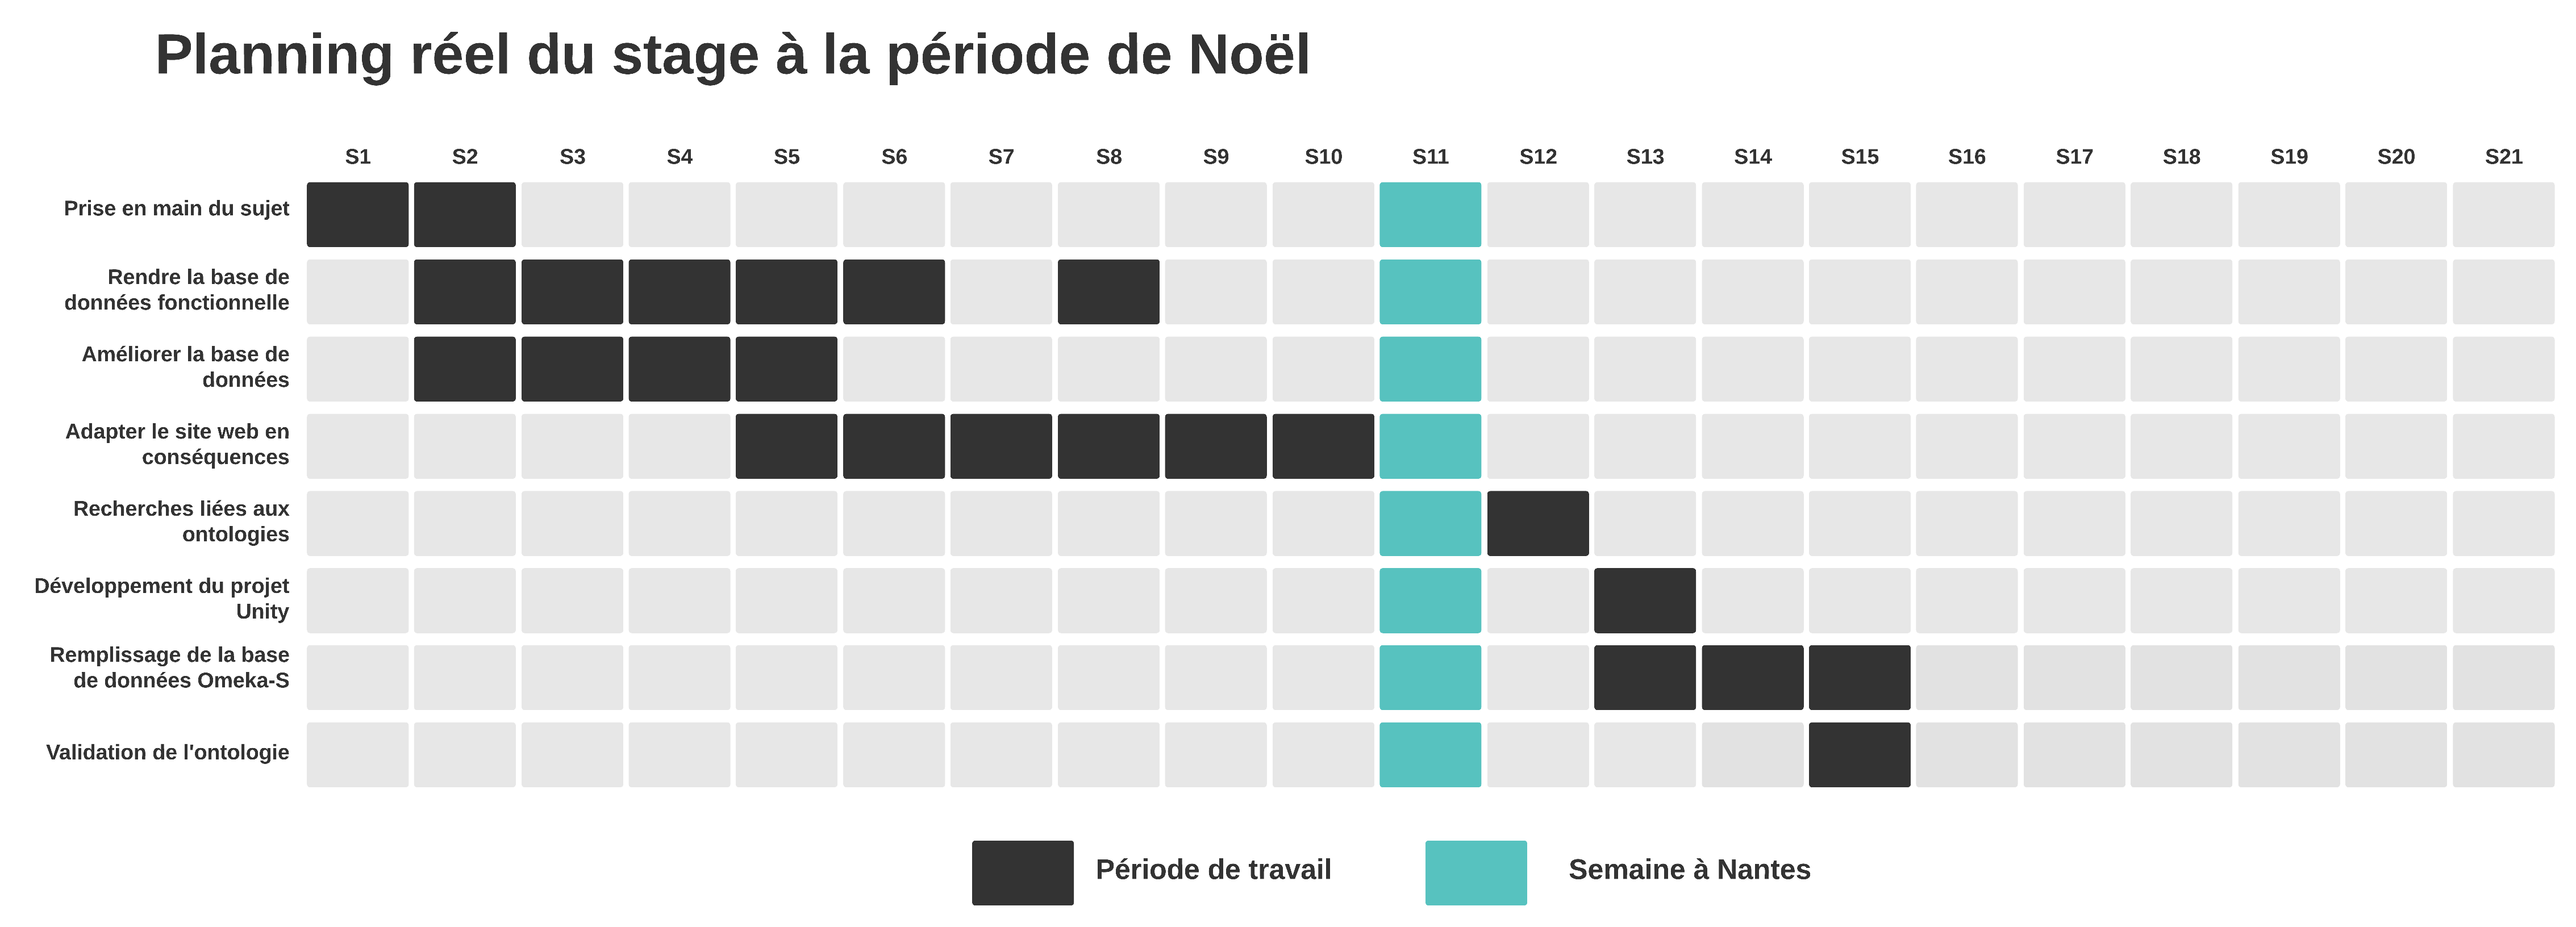
\includegraphics[width=1\textwidth]{assets/planning/planning_reel_noel.png}
    \caption{Planning réel à la période de Noël}
    \label{fig:planningReelNoel}
\end{figure}

\begin{figure} [H]
    \centering
    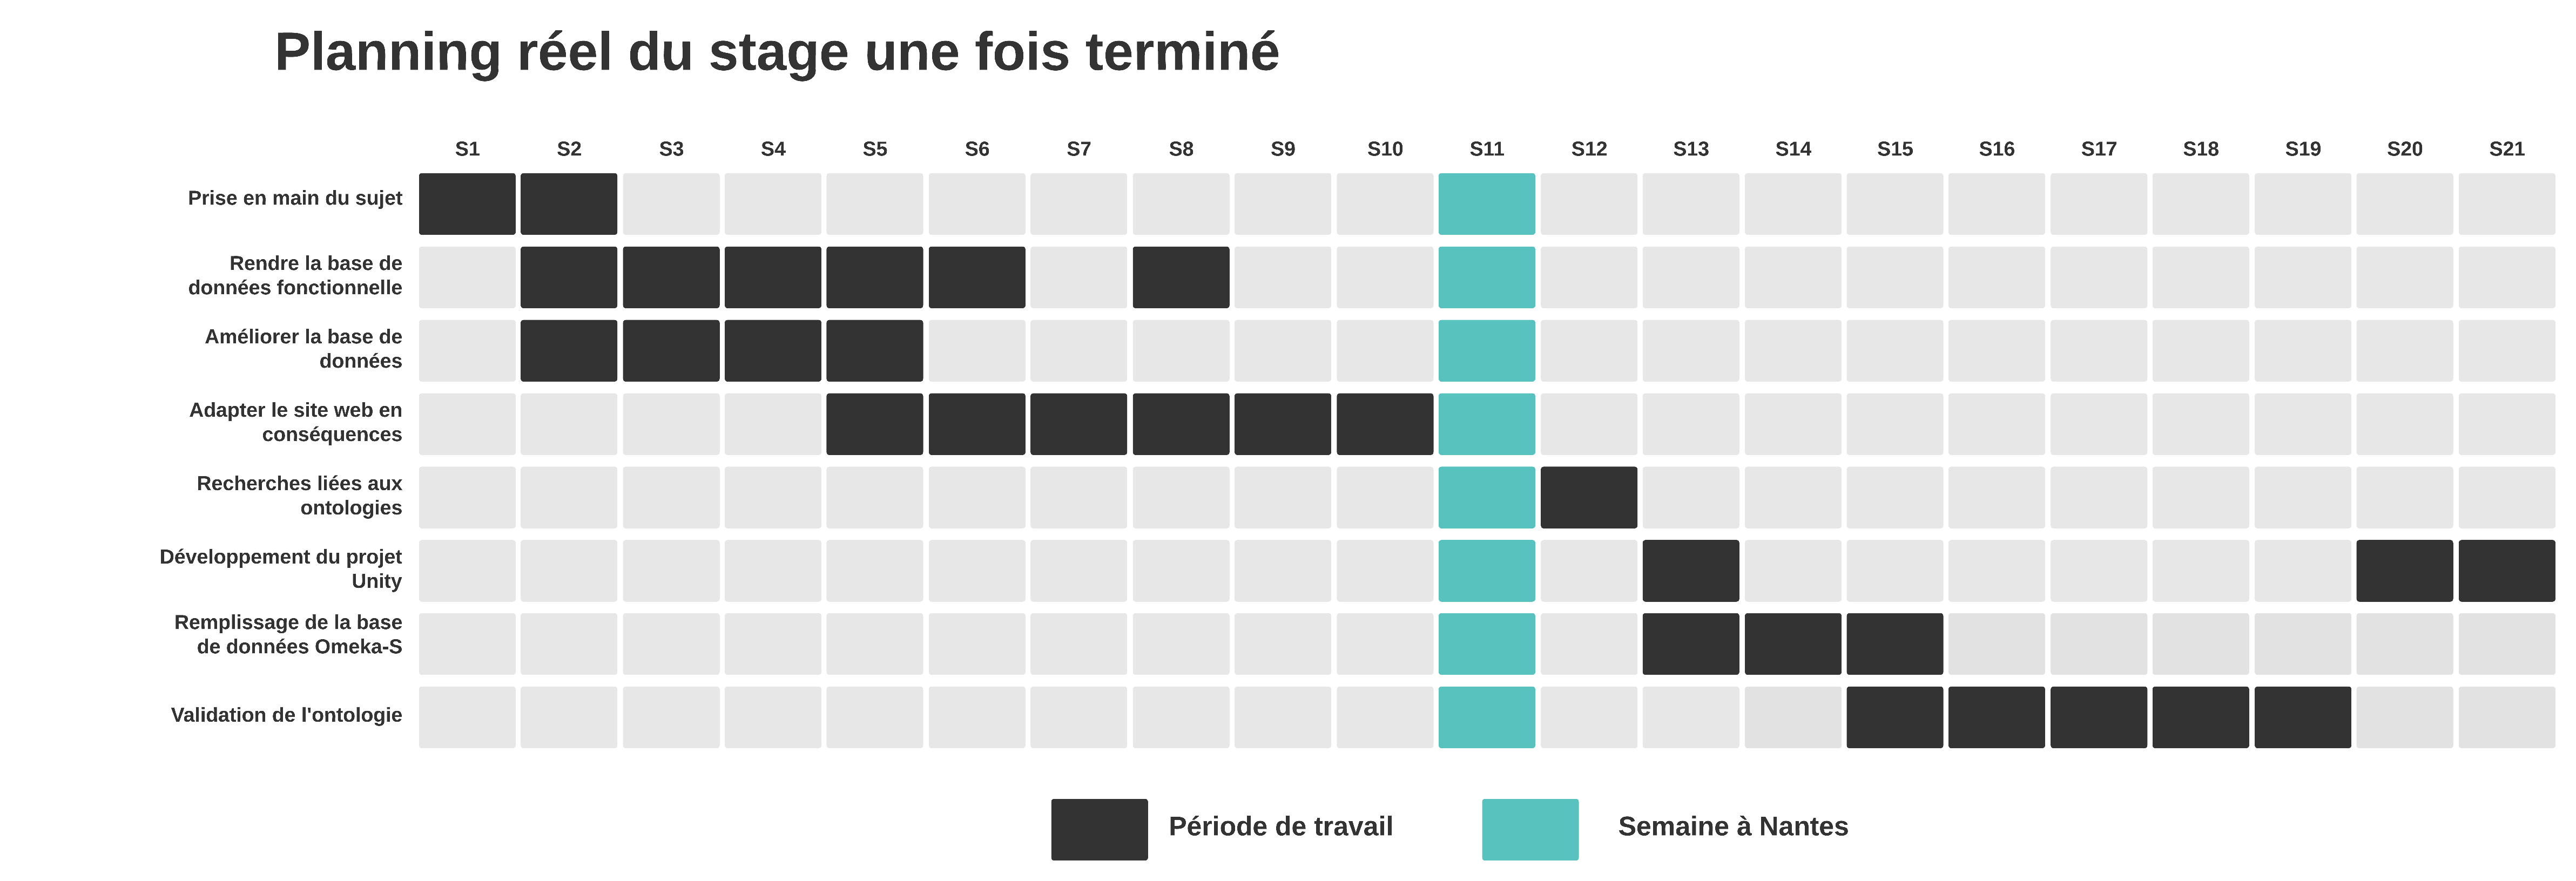
\includegraphics[width=1\textwidth]{assets/planning/planning_fin.png}
    \caption{Planning réel du stage une fois terminé}
    \label{fig:planningFin}
\end{figure}

